
\begin{figure}[t]
    \centering
    \begin{tabular}{ccc}
    \hspace{-5pt}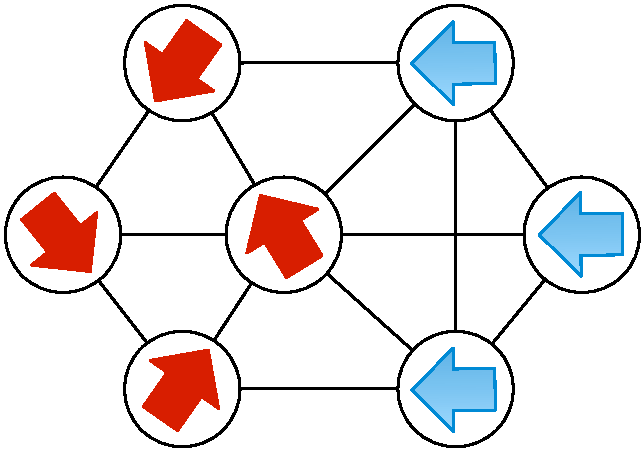
\includegraphics[width=1.3in]{../diagrams/bugs/loop.pdf}&
    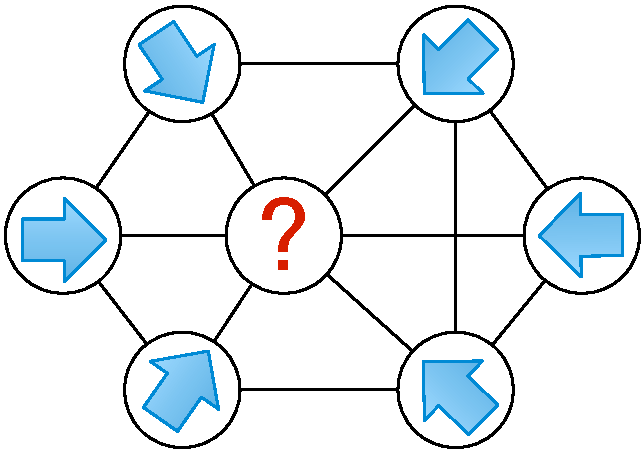
\includegraphics[width=1.3in]{../diagrams/bugs/dead_end.pdf}& \\
    {\bf (i) Loop}&{\bf (ii) Dead End}& \\
    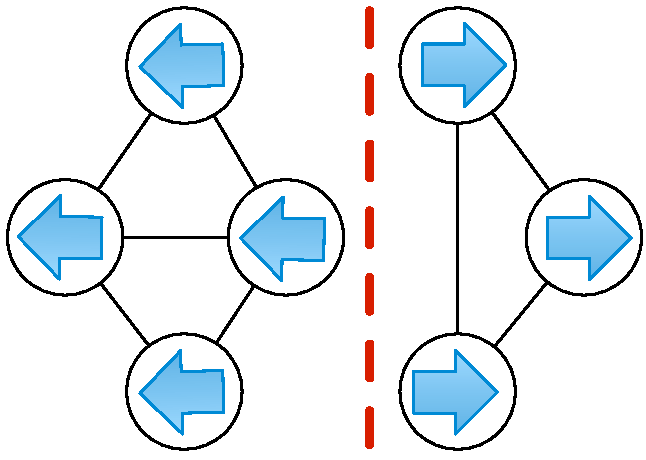
\includegraphics[width=1.3in]{../diagrams/bugs/partition.pdf}&
    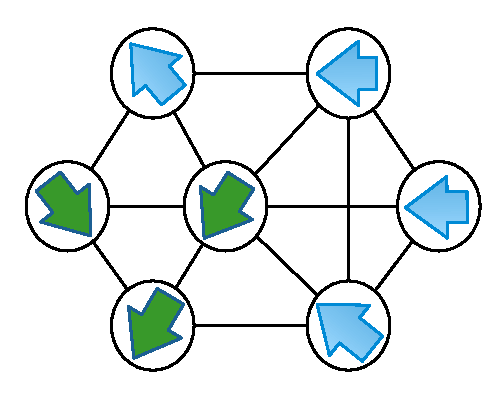
\includegraphics[width=1.3in]{../diagrams/bugs/routing_inconsistency.pdf}\\
     {\bf (iii) Partition}&{\bf (iv) Inconsistency}
    \end{tabular}
    \caption[]{\label{fig:generic_errors} Generic errors observed in
    networks.\vspace{-10pt}} 
\end{figure}


In this section we provide a taxonomy of common failure modes observed in
software-defined networks. We base our analysis on conversations with
researchers at Nicira~\cite{nicira}, a startup focused on developing a network operating
system for production SDN deployments~\cite{onix}. To the best of our
knowledge this is the first published analysis of common errors in SDN deployments\footnote{We were oh-so-close to getting the official bug reports out of Nicira by the class project deadline. We're waiting on CTO approval, but by SIGCOMM we'll actually be able to provide numbers and figures for each of these categories, as well as real anecdotes!}. 

Figure \ref{fig:generic_errors} depicts a set of errors which are
common to all networks. Loops (i) are a particularly common problem which
can result in significant packet loss and congestion. Dead ends, or
`blackholes` (ii) prevent packets entering the network from reaching their
final destination. Network partitions (iii) are a related problem where
some nodes in the network are not able to reach every other node. Finally, routing
inconsistencies (iv) cause packets to be treated under multiple, conflicting policies as
they traverse the network. 

In addition to generic network problems, error conditions exist which are
specific to the semantics of a particular control application. For example, a network
hosting web traffic may wish to guarantee that no incoming packet arrives
at a web server without first passing through a firewall. If a hardware
failure occurs, in-flight packet might violate this guarantee. As another
example, a load-balancing application may strive to ensure that no link
remains at full utilization more than 1\% of the time. If a sudden burst of
traffic enters the network, the application may be temporarily incapable
satisfying its constraints. 

Finally, a class of errors exists where the network does not behave as the
control application intends it to. A perfectly correct control application may
tell the NOS to route to traffic destined for a particular destination
out a particular egress, for example. A bug in the NOS itself, or a byzantine
failure in a network device might cause some traffic to leave an incorrect
egress.


These errors are typically the starting point for debugging: they are noticeable in the 
physical network, causing packets to be misrouted or lost.
However, noticing these errors in traditional networks often requires human involvement: our first challenge 
with \projectname{} is to classify these errors in terms of the mechanisms that \projectname{} must use and
understand to detect them independently.
Based on the Nicira reports, we classified each type of failure as one of three categories: physical misconfiguration (\S\ref{sec:dynamicmisconf}), correspondence violations (\S\ref{sec:correspond}), and consistency violations (\S\ref{sec:consistency}).


\subsection{Physical Misconfiguration}
\label{sec:dynamicmisconf}

The errors described in Figure \ref{fig:generic_errors} can all be detected with static checking
of FIB entries in the switches themselves.
Indeed, others~\cite{anteater} have developed efficient techniques to do so.


However, a challenge for \projectname{} is that these errors are not guaranteed to manifest 
at the time of verification.
Although traditional networks exhibit
low rates of configuration change, OpenFlow-based SDNs often have FIB entries generated dynamically on a per-flow basis. 
Thus, for traditional networks, a single verification of the
state of the network can catch most potential bugs. 
In contrast, software-defined networks can be more dynamic, and typically blur
the distinction between forwarding and auxiliary configuration.

For verification to be effective in this environment, static verification must
must span a larger set of possible output configurations for a given control
application: we must be able to inspect the network under numerous configurations, given varied configurations of active flows, arriving in different orders (and thus, varied FIB entries generated by the same SDN control stack).

\eat{ Discuss this later.
Moreover, there exist system executions in SDNs which result in error conditions that will never 
detected by a static checker. \colin{TODO: describe Justine's cool overlapping flow entries example}
}

\subsection{Correspondence Violation}
\label{sec:correspond}
Each layer of the SDN architecture
maintains its own model of the network state; the switches maintain forwarding
rules in TCAMs, the NOS represents the state of the switches in a graph-like data
structure, and control applications operate on 
a virtualized version of that graph. In theory, each layer's model should eventually
converge to a point where there is a one-to-one mapping 
between the other layers' models, but this does not always hold in practice.

This class of errors is particularly pernicious, as the 
virtualization layer of the NOS is often quite complex. Consider for example
that an entire datacenter network supporting 10s of thousands of hosts may be
treated as a single logical switch. When the control application makes a
configuration change to the logical switch, the NOS needs to carefully map this
configuration onto multiple physical switches along the path. Any mismapping in this
process may prevent the network from ever behaving exactly as the application intended.

Thus, errors may arise even when the physical network does not include loops, blackholes or the like: the network
may appear at first glance to function properly, when in reality it is performing differently than expected by the control application.
To detect this class of errors, \projectname{} must be able to inspect the datastructures representing switches and forwarding configurations at {\it each layer} of the SDN stack to verify correspondence.

\subsection{Consistency Violations}
\label{sec:consistency}
Production SDN deployments distribute the NOS
 across multiple servers to achieve fault-tolerance
and scalability. Distributed control gives rise to the same classes of coordination
and consistency bugs that affect general distributed systems. 

We note that two distinct classes of consistency violations occur in SDNs.
Transient consistency violations depend on the ordering of events in the system. For example,
if the  NOS pushes out a new forwarding policy
which involves multiple switches, in-flight packets may enter a
temporary forwarding loop while each of the switches converge on the new policy.
The effects of transient
consistency violations are noticeable distinct from persistent violations.

While our understanding of these problems is the least mature, we believe them to be the most
challenging class of errors for SDNs.

%\justine{is our goal to detect transient errors? it seems like detecting and 
%resolving transient errors is a good goal for a second project} \colin{Agreed.
%Both transient and persistent errors are important
%problems. But you go about dealing with them in very different ways. Not sure
%if the  distinction is valuable here (there are a million different
%distinctions we could make...)}



\eat{
\colin{Mention errors specific to OpenFlow? \eg overlapping flow entries. I
suppose that is really a form of routing inconsistency}
}


